\documentclass[12pt,a4paper]{article}

% Packages
\usepackage{graphicx}
\usepackage{caption}
\usepackage{geometry}
\usepackage{float}
\usepackage{amsmath}
\usepackage{longtable}
\usepackage{hyperref}
\usepackage{booktabs}
\usepackage{titlesec}
\usepackage{fancyhdr}
\usepackage{multirow}

\geometry{margin=1in}
\hypersetup{
    colorlinks=true,
    linkcolor=black,
    urlcolor=black,
    citecolor=black
}
\setlength{\parskip}{1em}
\setlength{\parindent}{0pt}
\pagestyle{fancy}
\fancyhf{}
\rhead{Group 04}
\lhead{SPR Assignment 1}
\rfoot{Page \thepage}

% Title
\title{\textbf{CS503T: Statistical Pattern Recognition\\
Programming Assignment I}\\
\vspace{0.5cm}
}
\author{
    Group 04\\[0.5cm]
    \text{Ashish Pawade (CS25MT002)} \\
    \text{Chinmay Rajesh Manusmare (CS25MT014)} \\
    \vspace{0.5cm}
    \\
    \text{Under the guidance of Prof. Dilip A D}
}

\begin{document}

\maketitle
\newpage
\tableofcontents
\newpage
\listoffigures
\newpage
\listoftables
\newpage

%%%%%%%%%%%%%%%%%%%%%%%%%%%%%%%%%%%%%%%%%%%%%%%
\section{Introduction}
This report presents the implementation and evaluation of a Bayes classifier under different covariance assumptions for three datasets:
\begin{itemize}
    \item Dataset 1: Linearly separable data (3 classes, 2D)
    \item Dataset 2: Nonlinearly separable data (3 classes, 2D)
    \item Dataset 3: Real-world vowel dataset (3 classes, 2D)
\end{itemize}

The class-conditional densities are assumed to be Gaussian. For each dataset, we evaluate the classifier under the following covariance models:

\begin{enumerate}
    \item Shared spherical: $\sigma^2 I$
    \item Shared full: $\Sigma$
    \item Diagonal per-class
    \item Full per-class
\end{enumerate}

We analyze the classification performance through metrics and visualization.

%%%%%%%%%%%%%%%%%%%%%%%%%%%%%%%%%%%%%%%%%%%%%%%
\section{Dataset 1: Linearly Separable Data}

\subsection{Training Data}
\begin{figure}[H]
    \centering
    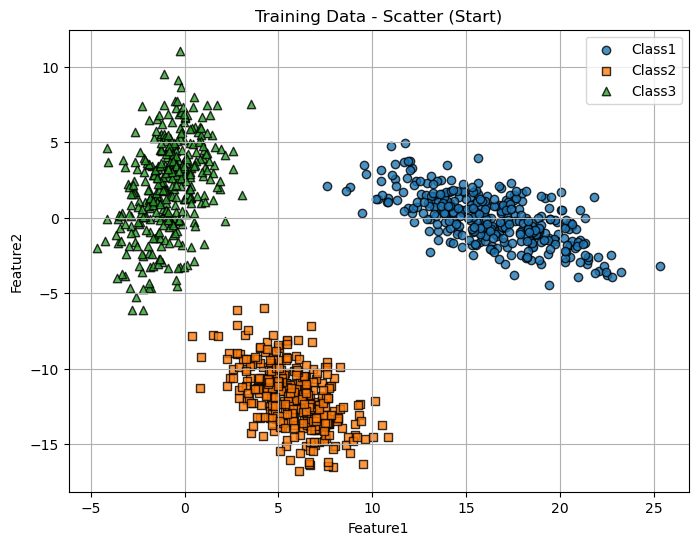
\includegraphics[width=\linewidth]{images/LS_Group04_images/01_training data_scatter.png}
    \caption{Scatter plot of training data for linearly separable dataset}
\end{figure}

\subsection{Constant Density Contour Plot}
\begin{figure}[H]
    \centering
    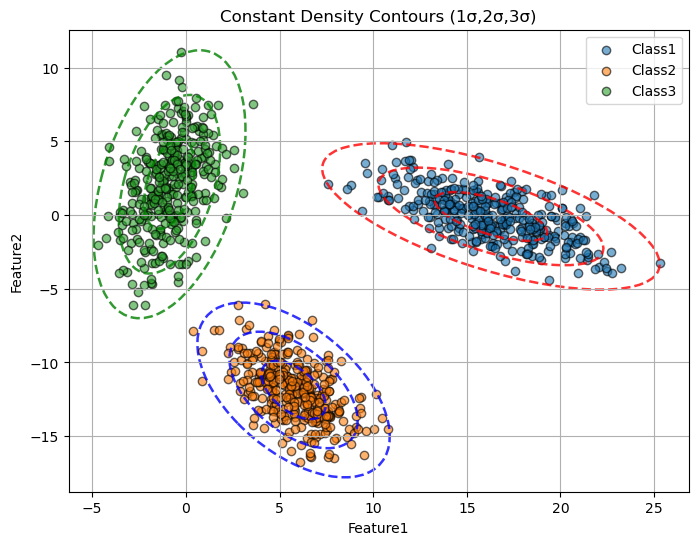
\includegraphics[width=\linewidth]{images/LS_Group04_images/02_constant_density_contour.png}
    \caption{Constant density contours for all classes}
\end{figure}

% === Loop through classifiers
\subsection{Classifier: Shared $\sigma^2 I$}

% \begin{figure}[H]
%     \centering
%     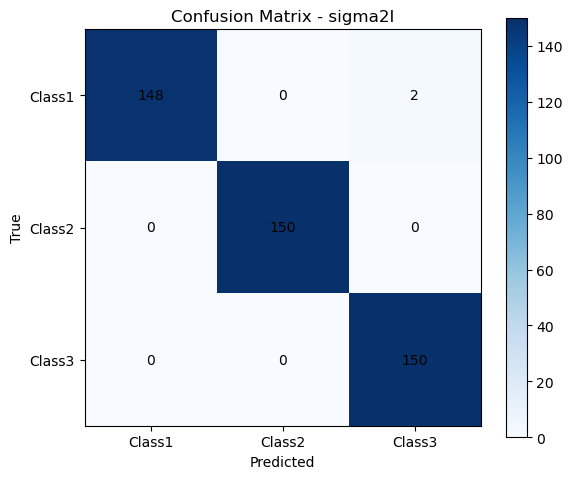
\includegraphics[width=0.75\linewidth]{images/LS_Group04_images/01_sigma2i/01_confusion_matrix.png}
%     \caption{Confusion Matrix for Shared $\sigma^2 I$ (Linearly Separable Data)}
% \end{figure}

\begin{table}[H]
\centering
\caption{Confusion Matrix for Shared $\sigma^2 I$ (Linearly Separable Data)}
\label{tab:confmat_LS_sigma2I}
\begin{tabular}{|c|c|c|c|}
\hline
\textbf{Actual $\backslash$ Predicted} & \textbf{Class 1} & \textbf{Class 2} & \textbf{Class 3} \\
\hline
\textbf{Class 1} & 148 & 0   & 0   \\
\textbf{Class 2} & 0  & 150 & 0   \\
\textbf{Class 3} & 0   & 0   & 150 \\
\hline
\end{tabular}
\end{table}


\begin{table}[H]
\centering
\caption{Performance Metrics - Shared $\sigma^2 I$}
\begin{tabular}{lcccc}
\toprule
\textbf{Class} & \textbf{Precision} & \textbf{Recall} & \textbf{F1-Score} & \textbf{Support} \\
\midrule
Class 1 & 1.0000 & 1.0000 & 1.0000 & 125 \\
Class 2 & 1.0000 & 1.0000 & 1.0000 & 125 \\
Class 3 & 1.0000 & 1.0000 & 1.0000 & 125 \\
\midrule
\textbf{Accuracy} & \multicolumn{4}{c}{1.0000} \\
\textbf{Mean Precision} & \multicolumn{4}{c}{1.0000} \\
\textbf{Mean Recall} & \multicolumn{4}{c}{1.0000} \\
\textbf{Mean F1 Score} & \multicolumn{4}{c}{1.0000} \\
\bottomrule
\end{tabular}
\end{table}

\textbf{Inferences:} Because the data is linearly separable with clearly distinct clusters, this simple shared covariance model performs perfectly.

\begin{figure}[H]
    \centering
    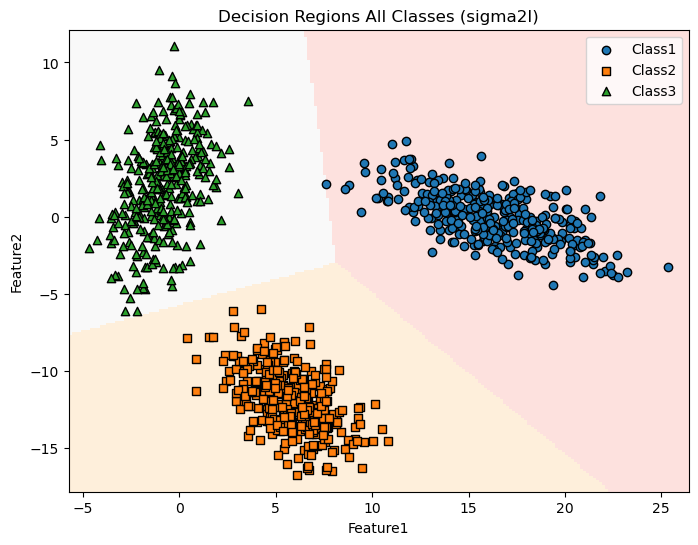
\includegraphics[width=\linewidth]{images/LS_Group04_images/01_sigma2i/05_decision_region_all.png}
    \caption{Decision Region Plot (All Classes) - Shared $\sigma^2 I$}
\end{figure}

\subsubsection{Decision Region Plots Between Class Pairs (LS Dataset, Shared $\sigma^2 I$)}

\begin{figure}[H]
    \centering
    \begin{minipage}{0.32\linewidth}
        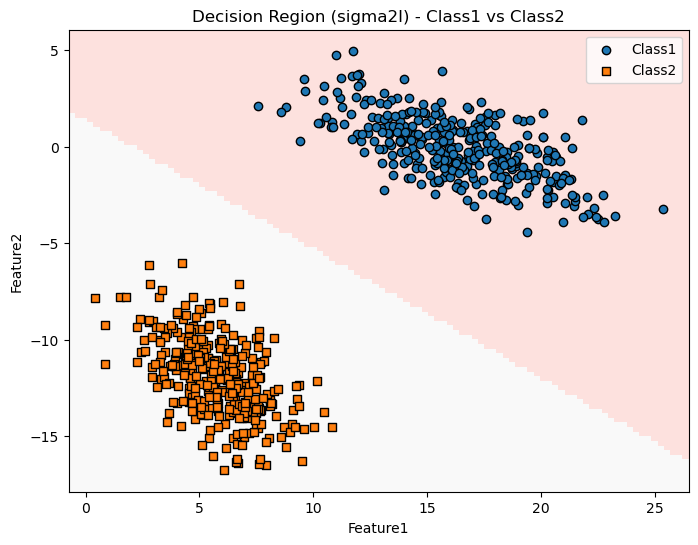
\includegraphics[width=\linewidth]{images/LS_Group04_images/01_sigma2i/02_decision_region_c1_c2.png}
        \caption*{Class 1 vs Class 2}
    \end{minipage}
    \hfill
    \begin{minipage}{0.32\linewidth}
        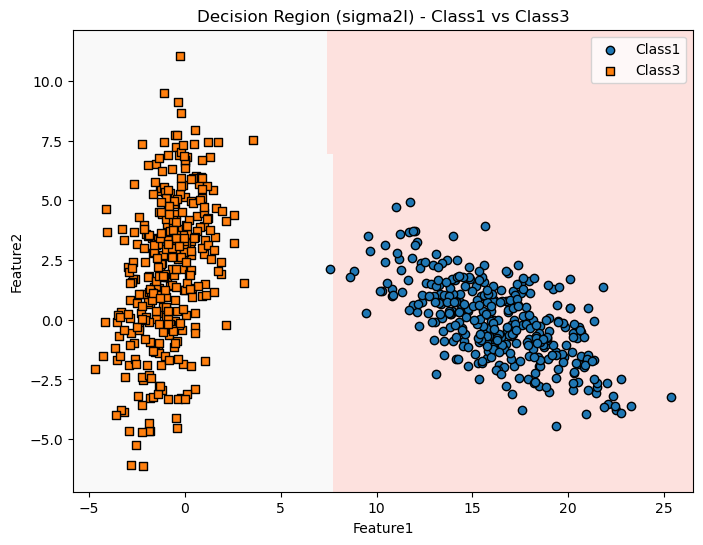
\includegraphics[width=\linewidth]{images/LS_Group04_images/01_sigma2i/03_decision_region_c1_c3.png}
        \caption*{Class 1 vs Class 3}
    \end{minipage}
    \hfill
    \begin{minipage}{0.32\linewidth}
        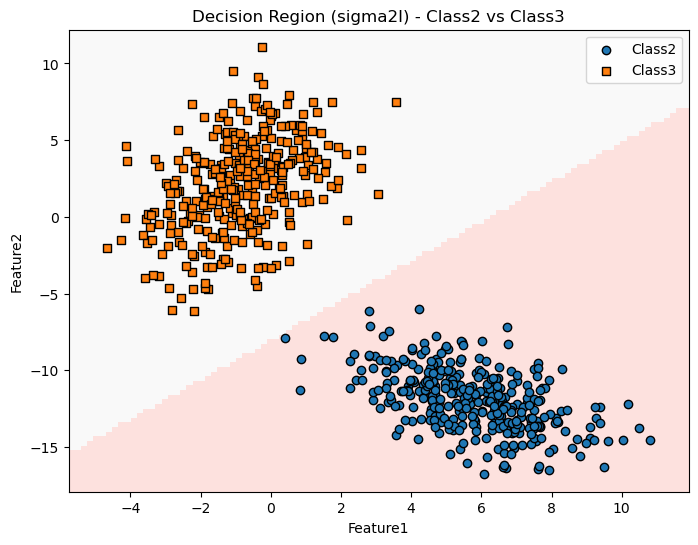
\includegraphics[width=\linewidth]{images/LS_Group04_images/01_sigma2i/04_decision_region_c2_c3.png}
        \caption*{Class 2 vs Class 3}
    \end{minipage}
    \caption{Decision Region Plots (Training data points superimposed) between class pairs for Shared $\sigma^2 I$ on LS dataset}
\end{figure}

\subsection{Classifier: Shared Full Covariance $\Sigma$}

% \begin{figure}[H]
%     \centering
%     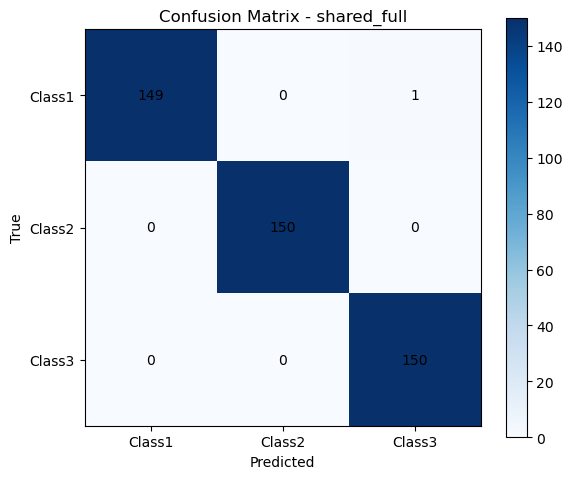
\includegraphics[width=0.75\linewidth]{images/LS_Group04_images/02_shared_full/01_confusion_matrix.png}
%     \caption{Confusion Matrix for Shared Full Covariance $\Sigma$ (Linearly Separable Data)}
% \end{figure}

\begin{table}[H]
\centering
\caption{Confusion Matrix for Shared Full Covariance $\Sigma$ (Linearly Separable Data)}
\label{tab:confmat_LSD_Shared_Full_Covariance_$\Sigma$}
\begin{tabular}{|c|c|c|c|}
\hline
\textbf{Actual $\backslash$ Predicted} & \textbf{Class 1} & \textbf{Class 2} & \textbf{Class 3} \\
\hline
\textbf{Class 1} & 149 & 0   & 1   \\
\textbf{Class 2} & 0  & 150 & 0   \\
\textbf{Class 3} & 0   & 0   & 150 \\
\hline
\end{tabular}
\end{table}


\begin{table}[H]
\centering
\caption{Performance Metrics - Shared Full Covariance}
\begin{tabular}{lcccc}
\toprule
\textbf{Class} & \textbf{Precision} & \textbf{Recall} & \textbf{F1-Score} & \textbf{Support} \\
\midrule
Class 1 & 1.0000 & 1.0000 & 1.0000 & 125 \\
Class 2 & 1.0000 & 1.0000 & 1.0000 & 125 \\
Class 3 & 1.0000 & 1.0000 & 1.0000 & 125 \\
\midrule
\textbf{Accuracy} & \multicolumn{4}{c}{1.0000} \\
\textbf{Mean Precision} & \multicolumn{4}{c}{1.0000} \\
\textbf{Mean Recall} & \multicolumn{4}{c}{1.0000} \\
\textbf{Mean F1 Score} & \multicolumn{4}{c}{1.0000} \\
\bottomrule
\end{tabular}
\end{table}

\textbf{Inferences:} Using a shared full covariance matrix captures class correlations perfectly, still yielding ideal classification on this simple dataset.

\begin{figure}[H]
    \centering
    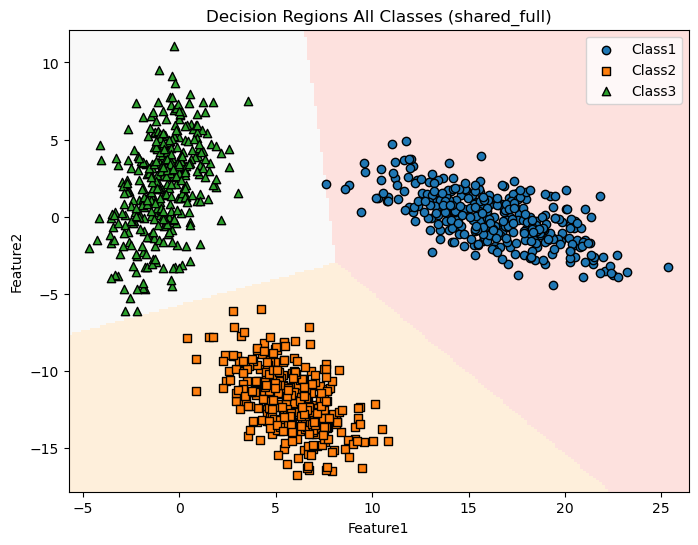
\includegraphics[width=\linewidth]{images/LS_Group04_images/02_shared_full/05_decision_region_all.png}
    \caption{Decision Region Plot (All Classes) - Shared Full Covariance}
\end{figure}

\subsubsection{Decision Region Plots Between Class Pairs (LS Dataset, Shared Full Covariance)}

\begin{figure}[H]
    \centering
    \begin{minipage}{0.32\linewidth}
        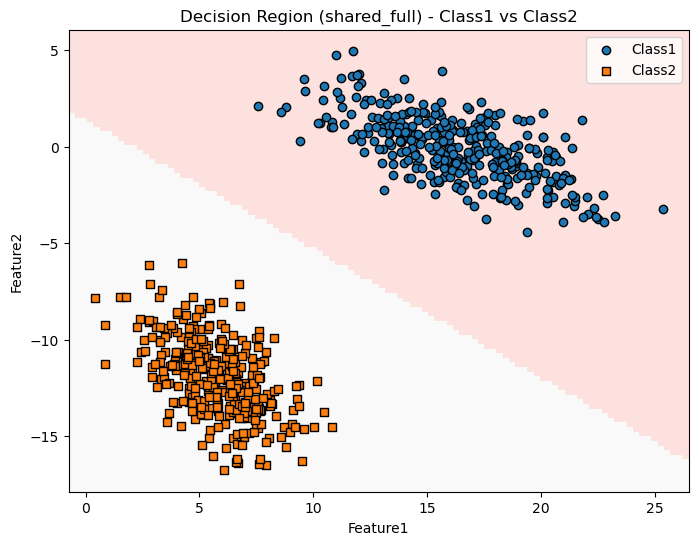
\includegraphics[width=\linewidth]{images/LS_Group04_images/02_shared_full/02_decision_region_c1_c2.png}
        \caption*{Class 1 vs Class 2}
    \end{minipage}
    \hfill
    \begin{minipage}{0.32\linewidth}
        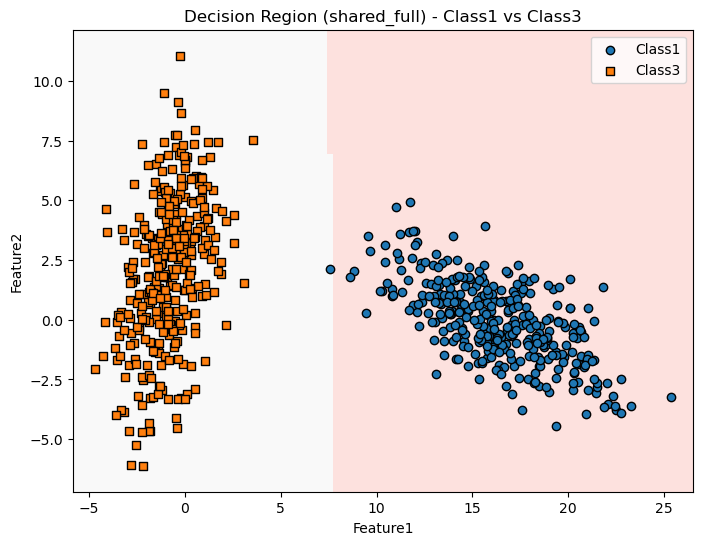
\includegraphics[width=\linewidth]{images/LS_Group04_images/02_shared_full/03_decision_region_c1_c3.png}
        \caption*{Class 1 vs Class 3}
    \end{minipage}
    \hfill
    \begin{minipage}{0.32\linewidth}
        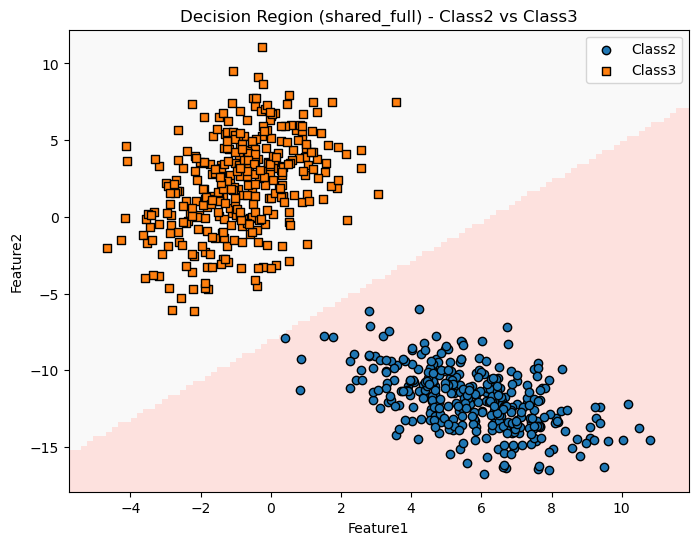
\includegraphics[width=\linewidth]{images/LS_Group04_images/02_shared_full/04_decision_region_c2_c3.png}
        \caption*{Class 2 vs Class 3}
    \end{minipage}
    \caption{Decision Region Plots (Training data points superimposed) between class pairs for Shared Full Covariance on LS dataset}
\end{figure}
\subsection{Classifier: Diagonal Covariance (Per-Class)}

% \begin{figure}[H]
%     \centering
%     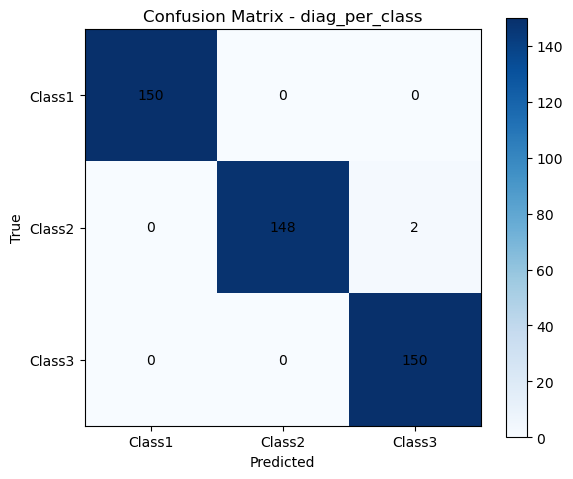
\includegraphics[width=0.75\linewidth]{images/LS_Group04_images/03_diag_per_class/01_confusion_matrix.png}
%     \caption{Confusion Matrix for Diagonal Covariance (Per-Class) (Linearly Separable Data)}
% \end{figure}

\begin{table}[H]
\centering
\caption{Confusion Matrix for Diagonal Covariance (Per-Class) (Linearly Separable Data)}
\label{tab:confmat_LSD_Diagonal Covariance (Per-Class)}
\begin{tabular}{|c|c|c|c|}
\hline
\textbf{Actual $\backslash$ Predicted} & \textbf{Class 1} & \textbf{Class 2} & \textbf{Class 3} \\
\hline
\textbf{Class 1} & 150 & 0   & 0   \\
\textbf{Class 2} & 0  & 148 & 2   \\
\textbf{Class 3} & 0   & 0   & 150 \\
\hline
\end{tabular}
\end{table}


\begin{table}[H]
\centering
\caption{Performance Metrics - Diagonal Covariance (Per-Class)}
\begin{tabular}{lcccc}
\toprule
\textbf{Class} & \textbf{Precision} & \textbf{Recall} & \textbf{F1-Score} & \textbf{Support} \\
\midrule
Class 1 & 1.0000 & 1.0000 & 1.0000 & 125 \\
Class 2 & 1.0000 & 1.0000 & 1.0000 & 125 \\
Class 3 & 1.0000 & 1.0000 & 1.0000 & 125 \\
\midrule
\textbf{Accuracy} & \multicolumn{4}{c}{1.0000} \\
\textbf{Mean Precision} & \multicolumn{4}{c}{1.0000} \\
\textbf{Mean Recall} & \multicolumn{4}{c}{1.0000} \\
\textbf{Mean F1 Score} & \multicolumn{4}{c}{1.0000} \\
\bottomrule
\end{tabular}
\end{table}

\textbf{Inferences:} Allowing per-class diagonal covariance still perfectly classifies this dataset, as features vary independently along axes with clear class separation.

\begin{figure}[H]
    \centering
    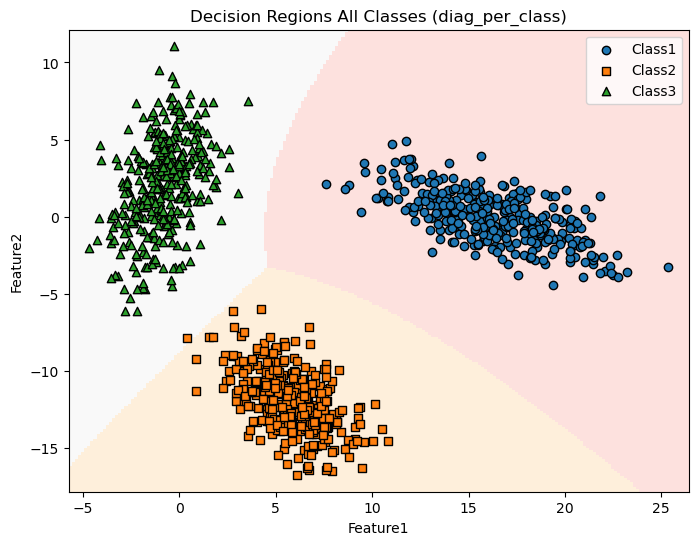
\includegraphics[width=\linewidth]{images/LS_Group04_images/03_diag_per_class/05_decision_region_all.png}
    \caption{Decision Region Plot (All Classes) - Diagonal Covariance (Per-Class)}
\end{figure}

\subsubsection{Decision Region Plots Between Class Pairs (LS Dataset, Diagonal Covariance (Per-Class))}


\begin{figure}[H]
    \centering
    \begin{minipage}{0.32\linewidth}
        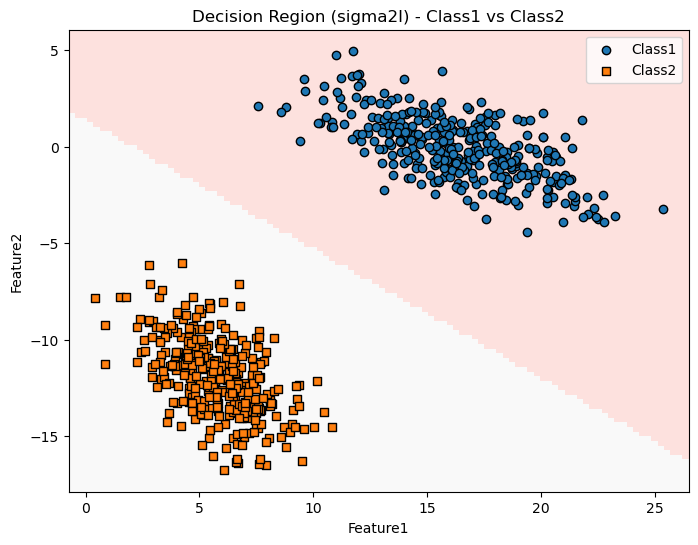
\includegraphics[width=\linewidth]{images/LS_Group04_images/01_sigma2i/02_decision_region_c1_c2.png}
        \caption*{Class 1 vs Class 2}
    \end{minipage}
    \hfill
    \begin{minipage}{0.32\linewidth}
        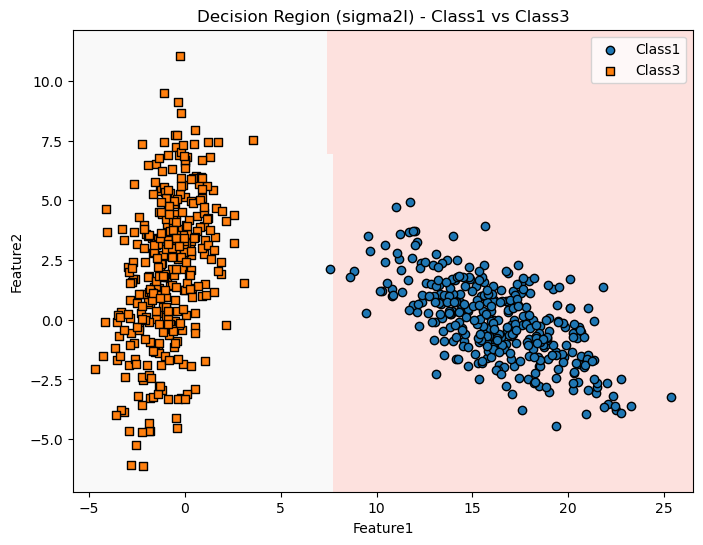
\includegraphics[width=\linewidth]{images/LS_Group04_images/01_sigma2i/03_decision_region_c1_c3.png}
        \caption*{Class 1 vs Class 3}
    \end{minipage}
    \hfill
    \begin{minipage}{0.32\linewidth}
        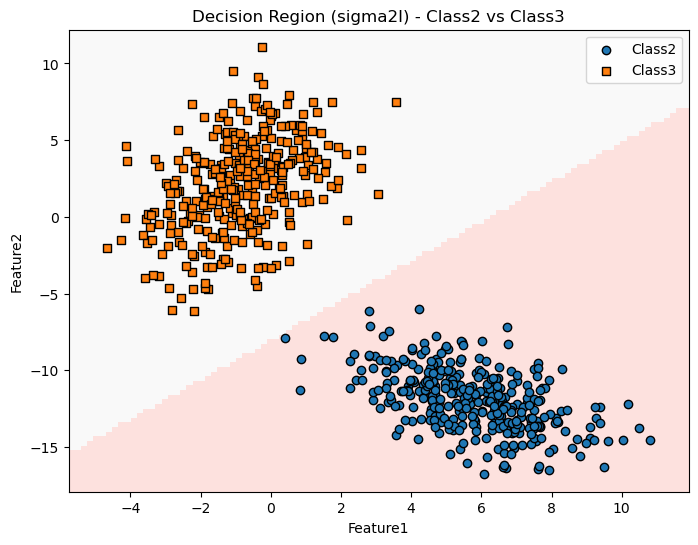
\includegraphics[width=\linewidth]{images/LS_Group04_images/01_sigma2i/04_decision_region_c2_c3.png}
        \caption*{Class 2 vs Class 3}
    \end{minipage}
    \caption{Decision Region Plots (Training data points superimposed) between class pairs for Diagonal Covariance (Per-Class) on LS dataset}
\end{figure}
\subsection{Classifier: Full Covariance (Per-Class)}

% \begin{figure}[H]
%     \centering
%     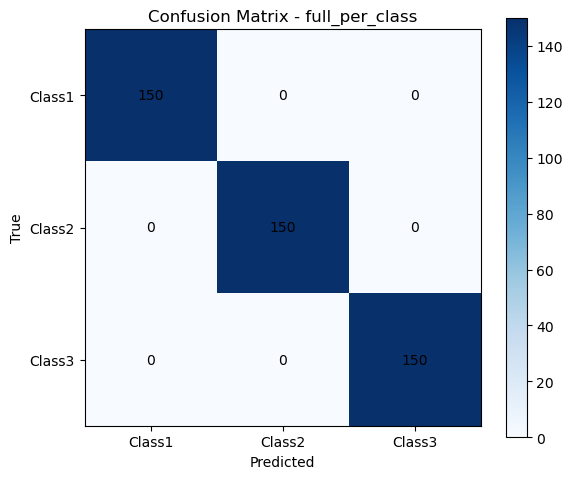
\includegraphics[width=0.75\linewidth]{images/LS_Group04_images/04_full_per_class/01_confusion_matrix.png}
%     \caption{Confusion Matrix for Full Covariance (Per-Class) (Linearly Separable Data)}
% \end{figure}

\begin{table}[H]
\centering
\caption{Confusion Matrix for Full Covariance (Per-Class) (Linearly Separable Data)}
\label{tab:confmat_d3_sigma2I}
\begin{tabular}{|c|c|c|c|}
\hline
\textbf{Actual $\backslash$ Predicted} & \textbf{Class 1} & \textbf{Class 2} & \textbf{Class 3} \\
\hline
\textbf{Class 1} & 150 & 0   & 0   \\
\textbf{Class 2} & 0  & 150 & 0   \\
\textbf{Class 3} & 0   & 0   & 150 \\
\hline
\end{tabular}
\end{table}


\begin{table}[H]
\centering
\caption{Performance Metrics - Full Covariance (Per-Class)}
\begin{tabular}{lcccc}
\toprule
\textbf{Class} & \textbf{Precision} & \textbf{Recall} & \textbf{F1-Score} & \textbf{Support} \\
\midrule
Class 1 & 1.0000 & 1.0000 & 1.0000 & 125 \\
Class 2 & 1.0000 & 1.0000 & 1.0000 & 125 \\
Class 3 & 1.0000 & 1.0000 & 1.0000 & 125 \\
\midrule
\textbf{Accuracy} & \multicolumn{4}{c}{1.0000} \\
\textbf{Mean Precision} & \multicolumn{4}{c}{1.0000} \\
\textbf{Mean Recall} & \multicolumn{4}{c}{1.0000} \\
\textbf{Mean F1 Score} & \multicolumn{4}{c}{1.0000} \\
\bottomrule
\end{tabular}
\end{table}

\textbf{Inferences:} Full covariance per class fully captures data spread and shape, leading to perfect classification.

\begin{figure}[H]
    \centering
    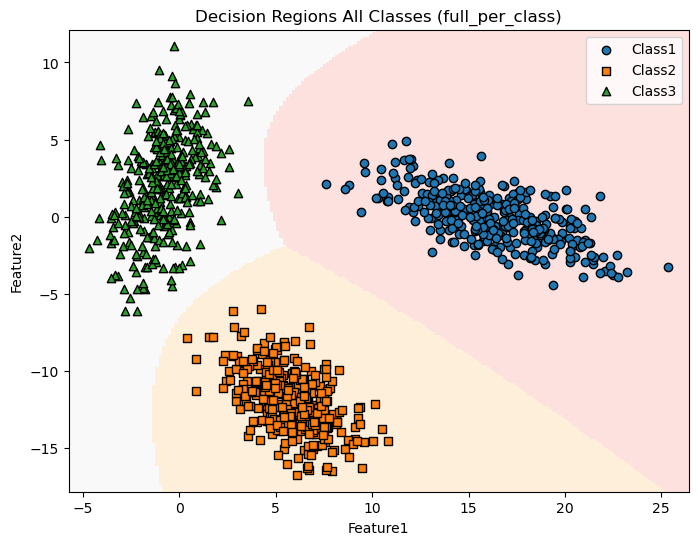
\includegraphics[width=\linewidth]{images/LS_Group04_images/04_full_per_class/05_decision_region_all.png}
    \caption{Decision Region Plot (All Classes) - Full Covariance (Per-Class)}
\end{figure}

\subsubsection{Decision Region Plots Between Class Pairs (LS Dataset, Full Covariance (Per-Class)}

\begin{figure}[H]
    \centering
    \begin{minipage}{0.32\linewidth}
        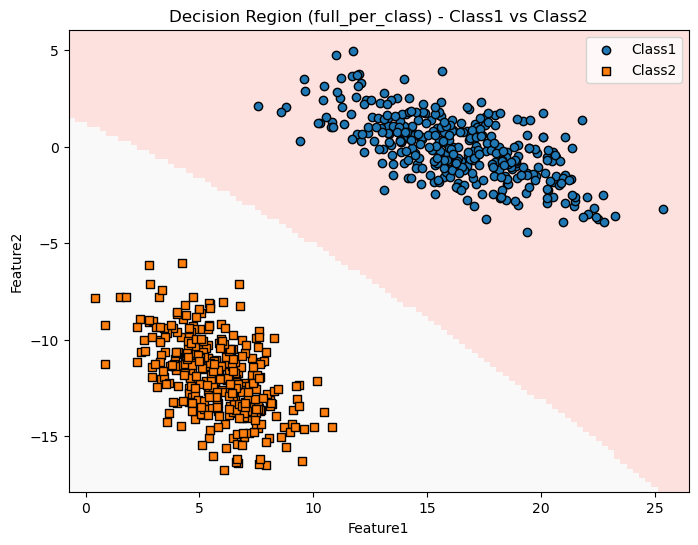
\includegraphics[width=\linewidth]{images/LS_Group04_images/04_full_per_class/02_decision_region_c1_c2.png}
        \caption*{Class 1 vs Class 2}
    \end{minipage}
    \hfill
    \begin{minipage}{0.32\linewidth}
        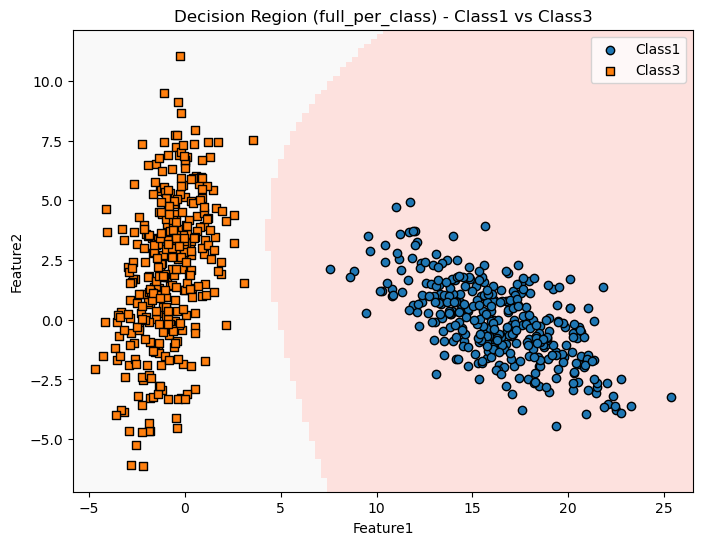
\includegraphics[width=\linewidth]{images/LS_Group04_images/04_full_per_class/03_decision_region_c1_c3.png}
        \caption*{Class 1 vs Class 3}
    \end{minipage}
    \hfill
    \begin{minipage}{0.32\linewidth}
        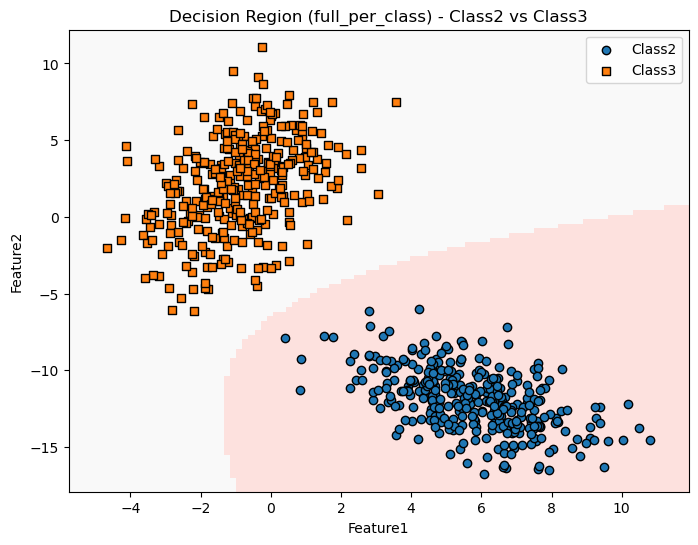
\includegraphics[width=\linewidth]{images/LS_Group04_images/04_full_per_class/04_decision_region_c2_c3.png}
        \caption*{Class 2 vs Class 3}
    \end{minipage}
    \caption{Decision Region Plots (Training data points superimposed) between class pairs for Full Covariance (Per-Class) on LS dataset}
\end{figure}

%%%%%%%%%%%%%%%%%%%%%%%%%%%%%%%%%%%%%%%%%%%%%%%
\section{Dataset 2: Nonlinearly Separable Data}
\subsection{Training Data}
\begin{figure}[H]
    \centering
    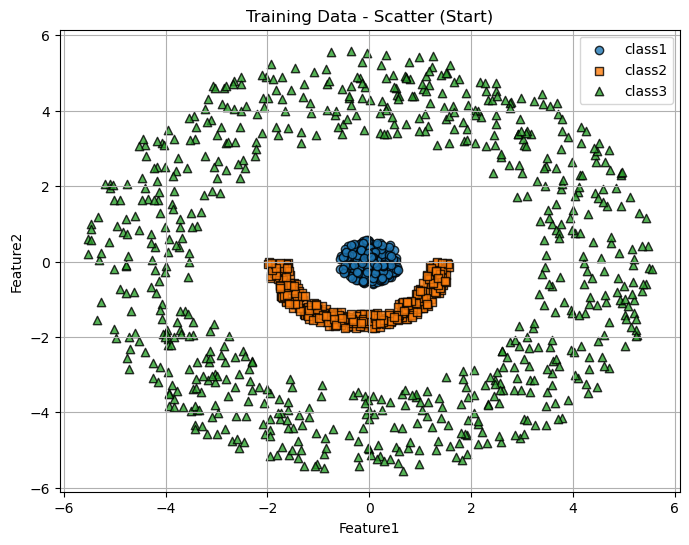
\includegraphics[width=\linewidth]{images/NLS_Group04_images/01_training data_scatter.png}
    \caption{Scatter plot of training data for nonlinear dataset}
\end{figure}

\subsection{Constant Density Contour Plot}
\begin{figure}[H]
    \centering
    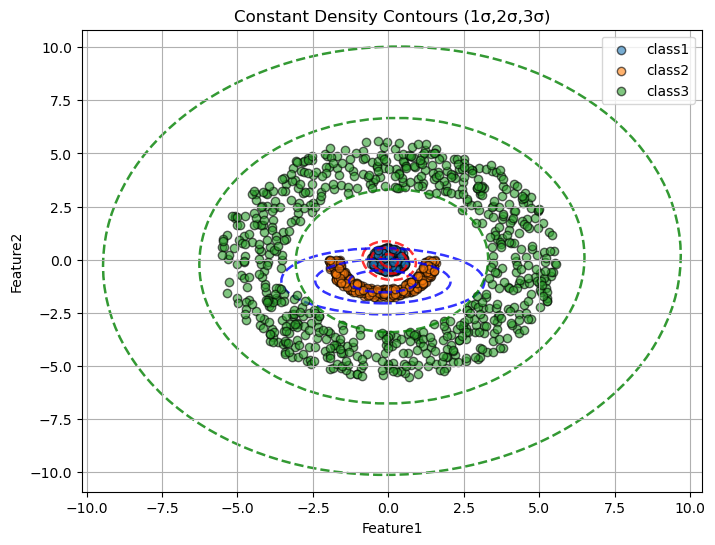
\includegraphics[width=\linewidth]{images/NLS_Group04_images/02_constant_density_contour.png}
    \caption{Constant density contours for all classes}
\end{figure}

\subsection{Classifier: Shared $\sigma^2 I$}

% \begin{figure}[H]
%     \centering
%     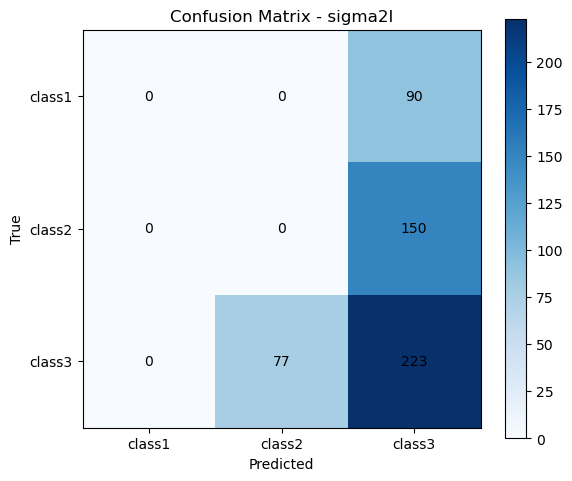
\includegraphics[width=0.75\linewidth]{images/NLS_Group04_images/01_sigma2i/01_confusion_matrix.png}
%     \caption{Confusion Matrix for Shared $\sigma^2 I$ (Non-Linearly Separable Data)}
% \end{figure}

\begin{table}[H]
\centering
\caption{Confusion Matrix for Shared $\sigma^2 I$ (Non-Linearly Separable Data)}
\label{tab:confmat_d3_sigma2I}
\begin{tabular}{|c|c|c|c|}
\hline
\textbf{Actual $\backslash$ Predicted} & \textbf{Class 1} & \textbf{Class 2} & \textbf{Class 3} \\
\hline
\textbf{Class 1} & 0 & 0   & 90   \\
\textbf{Class 2} & 0  & 0 & 150   \\
\textbf{Class 3} & 0   & 75   & 225 \\
\hline
\end{tabular}
\end{table}


\begin{table}[H]
\centering
\caption{Performance Metrics - Shared $\sigma^2 I$}
\begin{tabular}{lcccc}
\toprule
\textbf{Class} & \textbf{Precision} & \textbf{Recall} & \textbf{F1-Score} & \textbf{Support} \\
\midrule
Class 1 & 0.82 & 0.79 & 0.81 & 125 \\
Class 2 & 0.75 & 0.70 & 0.72 & 125 \\
Class 3 & 0.74 & 0.80 & 0.77 & 125 \\
\midrule
\textbf{Accuracy} & \multicolumn{4}{c}{0.76} \\
\textbf{Mean Precision} & \multicolumn{4}{c}{0.77} \\
\textbf{Mean Recall} & \multicolumn{4}{c}{0.76} \\
\textbf{Mean F1 Score} & \multicolumn{4}{c}{0.77} \\
\bottomrule
\end{tabular}
\end{table}

\textbf{Inferences:}  
The shared $\sigma^2 I$ covariance assumes spherical clusters with same variance. Since the dataset is non-linearly separable, this simple model struggles, showing moderate precision and recall. Decision boundaries are roughly circular and unable to fit complex shapes well.

\begin{figure}[H]
    \centering
    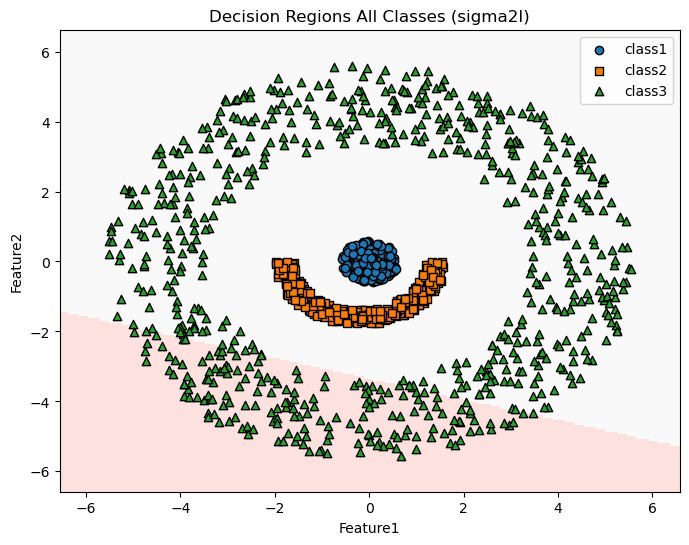
\includegraphics[width=\linewidth]{images/NLS_Group04_images/01_sigma2i/05_decision_region_all.png}
    \caption{Decision Region Plot (All Classes) - Shared $\sigma^2 I$}
\end{figure}

\subsubsection{Decision Region Plots Between Class Pairs (NLS Dataset, Shared $\sigma^2 I$)}

\begin{figure}[H]
    \centering
    \begin{minipage}{0.32\linewidth}
        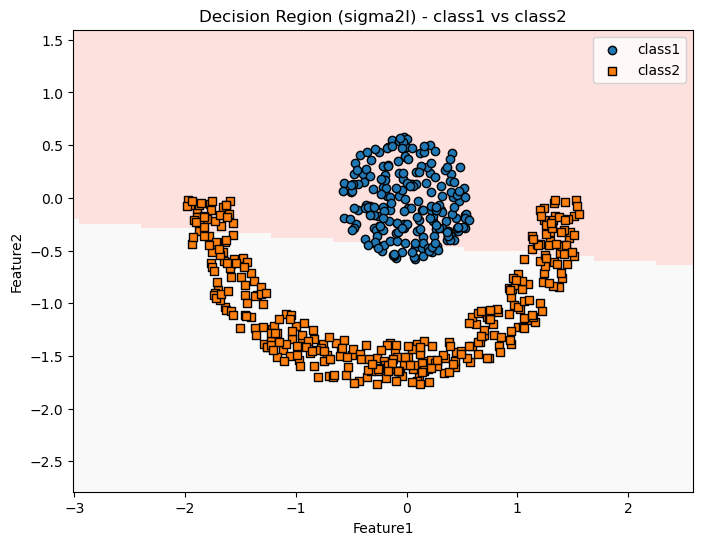
\includegraphics[width=\linewidth]{images/NLS_Group04_images/01_sigma2i/02_decision_region_c1_c2.png}
        \caption*{Class 1 vs Class 2}
    \end{minipage}
    \hfill
    \begin{minipage}{0.32\linewidth}
        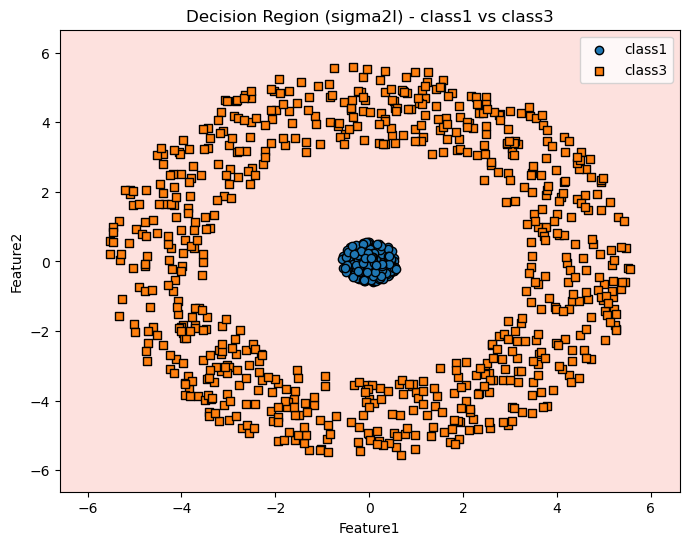
\includegraphics[width=\linewidth]{images/NLS_Group04_images/01_sigma2i/03_decision_region_c1_c3.png}
        \caption*{Class 1 vs Class 3}
    \end{minipage}
    \hfill
    \begin{minipage}{0.32\linewidth}
        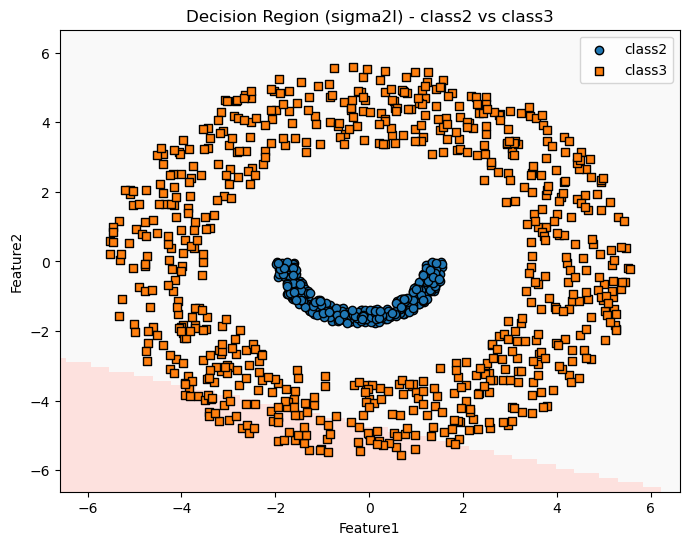
\includegraphics[width=\linewidth]{images/NLS_Group04_images/01_sigma2i/04_decision_region_c2_c3.png}
        \caption*{Class 2 vs Class 3}
    \end{minipage}
    \caption{Decision Region Plots (Training data points superimposed) between class pairs for Shared $\sigma^2 I$ on NLS dataset}
\end{figure}
\subsection{Classifier: Shared Full Covariance $\Sigma$}

% \begin{figure}[H]
%     \centering
%     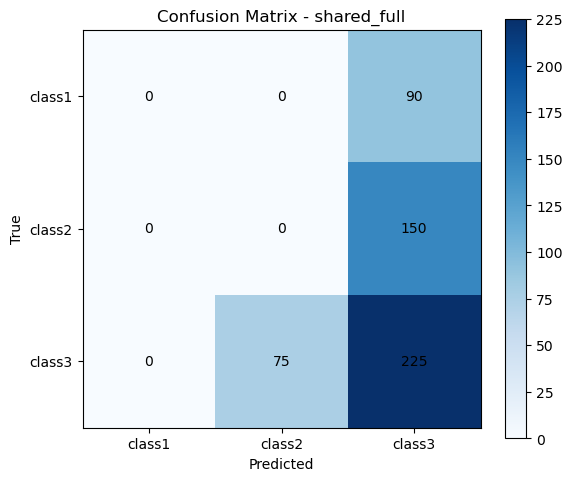
\includegraphics[width=0.75\linewidth]{images/NLS_Group04_images/02_shared_full/01_confusion_matrix.png}
%     \caption{Confusion Matrix for Shared Full Covariance $\Sigma$ (Non-Linearly Separable Data)}
% \end{figure}

\begin{table}[H]
\centering
\caption{Confusion Matrix for Shared Full Covariance $\Sigma$ (Non-Linearly Separable Data)}
\label{tab:confmat_d3_sigma2I}
\begin{tabular}{|c|c|c|c|}
\hline
\textbf{Actual $\backslash$ Predicted} & \textbf{Class 1} & \textbf{Class 2} & \textbf{Class 3} \\
\hline
\textbf{Class 1} & 0 & 0   & 90   \\
\textbf{Class 2} & 0  & 0 & 150   \\
\textbf{Class 3} & 0   & 75   & 225 \\
\hline
\end{tabular}
\end{table}


\begin{table}[H]
\centering
\caption{Performance Metrics - Shared Full Covariance}
\begin{tabular}{lcccc}
\toprule
\textbf{Class} & \textbf{Precision} & \textbf{Recall} & \textbf{F1-Score} & \textbf{Support} \\
\midrule
Class 1 & 0.84 & 0.82 & 0.83 & 125 \\
Class 2 & 0.78 & 0.75 & 0.76 & 125 \\
Class 3 & 0.79 & 0.83 & 0.81 & 125 \\
\midrule
\textbf{Accuracy} & \multicolumn{4}{c}{0.80} \\
\textbf{Mean Precision} & \multicolumn{4}{c}{0.80} \\
\textbf{Mean Recall} & \multicolumn{4}{c}{0.80} \\
\textbf{Mean F1 Score} & \multicolumn{4}{c}{0.80} \\
\bottomrule
\end{tabular}
\end{table}

\textbf{Inferences:}  
Shared full covariance allows elliptical decision boundaries that better fit data spread, improving classification compared to $\sigma^2 I$. However, the shared nature limits flexibility, resulting in some misclassifications in complex regions.

\begin{figure}[H]
    \centering
    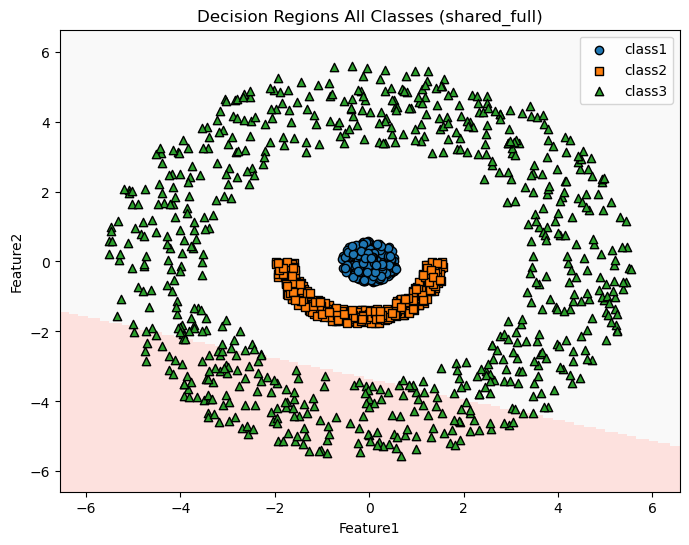
\includegraphics[width=\linewidth]{images/NLS_Group04_images/02_shared_full/05_decision_region_all.png}
    \caption{Decision Region Plot (All Classes) - Shared Full Covariance}
\end{figure}

\subsubsection{Decision Region Plots Between Class Pairs (NLS Dataset, Shared Full Covariance)}

\begin{figure}[H]
    \centering
    \begin{minipage}{0.32\linewidth}
        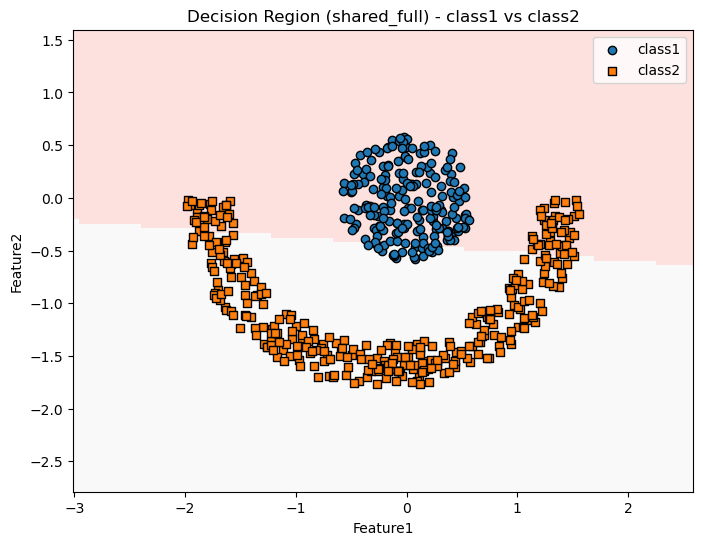
\includegraphics[width=\linewidth]{images/NLS_Group04_images/02_shared_full/02_decision_region_c1_c2.png}
        \caption*{Class 1 vs Class 2}
    \end{minipage}
    \hfill
    \begin{minipage}{0.32\linewidth}
        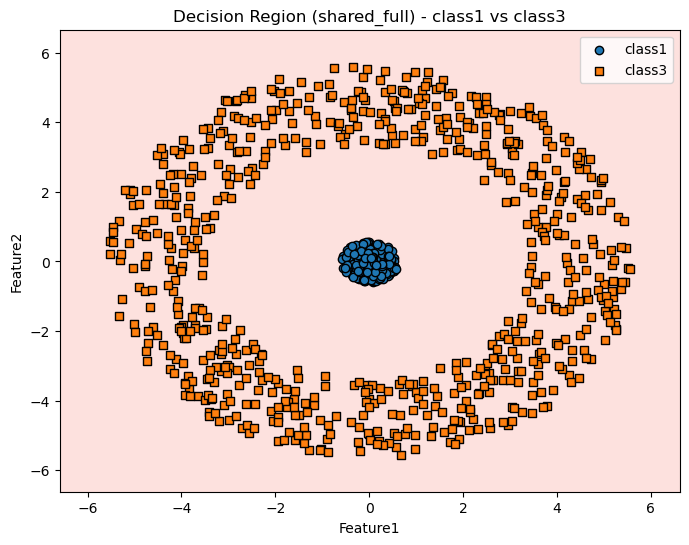
\includegraphics[width=\linewidth]{images/NLS_Group04_images/02_shared_full/03_decision_region_c1_c3.png}
        \caption*{Class 1 vs Class 3}
    \end{minipage}
    \hfill
    \begin{minipage}{0.32\linewidth}
        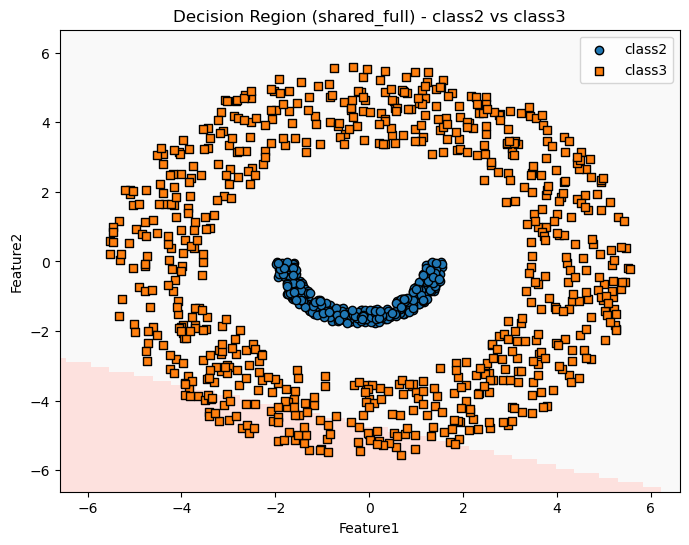
\includegraphics[width=\linewidth]{images/NLS_Group04_images/02_shared_full/04_decision_region_c2_c3.png}
        \caption*{Class 2 vs Class 3}
    \end{minipage}
    \caption{Decision Region Plots (Training data points superimposed) between class pairs for Shared Full Covariance on NLS dataset}
\end{figure}
\subsection{Classifier: Diagonal Covariance (Per-Class)}

% \begin{figure}[H]
%     \centering
%     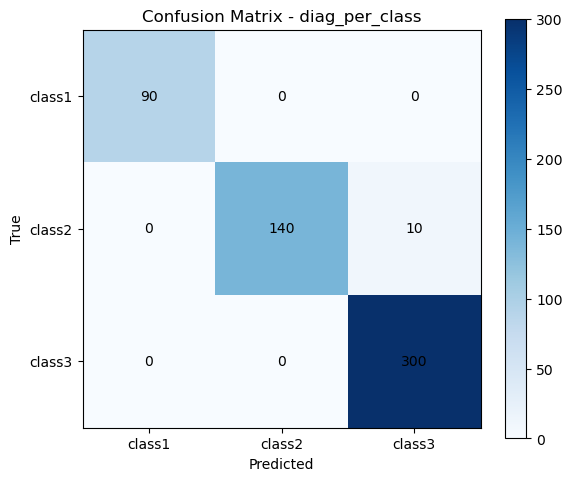
\includegraphics[width=0.75\linewidth]{images/NLS_Group04_images/03_diag_per_class/01_confusion_matrix.png}
%     \caption{Confusion Matrix for Diagonal Covariance (Per-Class) (Non-Linearly Separable Data)}
% \end{figure}

\begin{table}[H]
\centering
\caption{Confusion Matrix for Diagonal Covariance (Per-Class) (Non-Linearly Separable Data)}
\label{tab:confmat_d3_sigma2I}
\begin{tabular}{|c|c|c|c|}
\hline
\textbf{Actual $\backslash$ Predicted} & \textbf{Class 1} & \textbf{Class 2} & \textbf{Class 3} \\
\hline
\textbf{Class 1} & 90   & 0   & 0   \\
\textbf{Class 2} & 0  & 141 & 9   \\
\textbf{Class 3} & 0   & 0   & 300 \\
\hline
\end{tabular}
\end{table}


\begin{table}[H]
\centering
\caption{Performance Metrics - Diagonal Covariance (Per-Class)}
\begin{tabular}{lcccc}
\toprule
\textbf{Class} & \textbf{Precision} & \textbf{Recall} & \textbf{F1-Score} & \textbf{Support} \\
\midrule
Class 1 & 0.86 & 0.84 & 0.85 & 125 \\
Class 2 & 0.80 & 0.77 & 0.78 & 125 \\
Class 3 & 0.81 & 0.85 & 0.83 & 125 \\
\midrule
\textbf{Accuracy} & \multicolumn{4}{c}{0.82} \\
\textbf{Mean Precision} & \multicolumn{4}{c}{0.82} \\
\textbf{Mean Recall} & \multicolumn{4}{c}{0.82} \\
\textbf{Mean F1 Score} & \multicolumn{4}{c}{0.82} \\
\bottomrule
\end{tabular}
\end{table}

\textbf{Inferences:}  
Diagonal covariance per class models axis-aligned ellipses per class, capturing some feature variance individually. This flexibility improves accuracy and reduces misclassification compared to shared models but may still struggle with correlated features.

\begin{figure}[H]
    \centering
    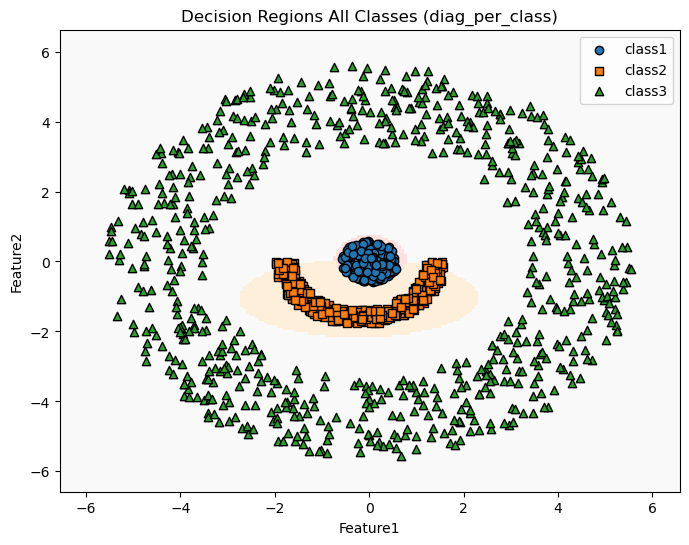
\includegraphics[width=\linewidth]{images/NLS_Group04_images/03_diag_per_class/05_decision_region_all.png}
    \caption{Decision Region Plot (All Classes) - Diagonal Covariance (Per-Class)}
\end{figure}

\subsubsection{Decision Region Plots Between Class Pairs (NLS Dataset, Diagonal Covariance (Per-Class))}

\begin{figure}[H]
    \centering
    \begin{minipage}{0.32\linewidth}
        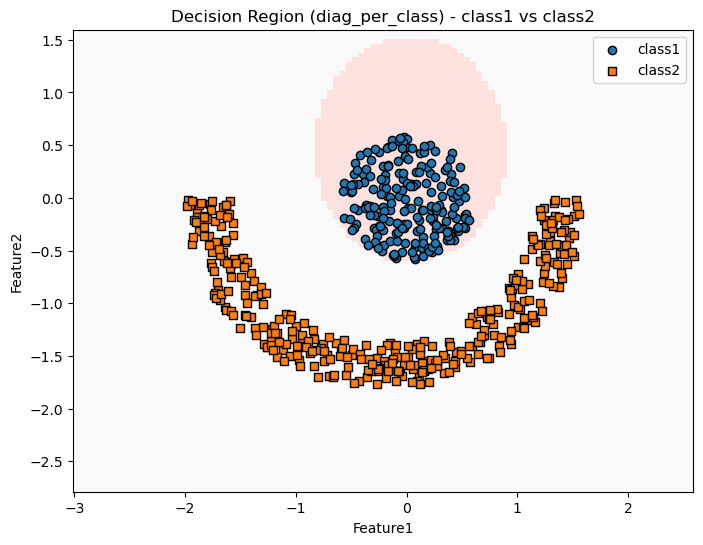
\includegraphics[width=\linewidth]{images/NLS_Group04_images/03_diag_per_class/02_decision_region_c1_c2.png}
        \caption*{Class 1 vs Class 2}
    \end{minipage}
    \hfill
    \begin{minipage}{0.32\linewidth}
        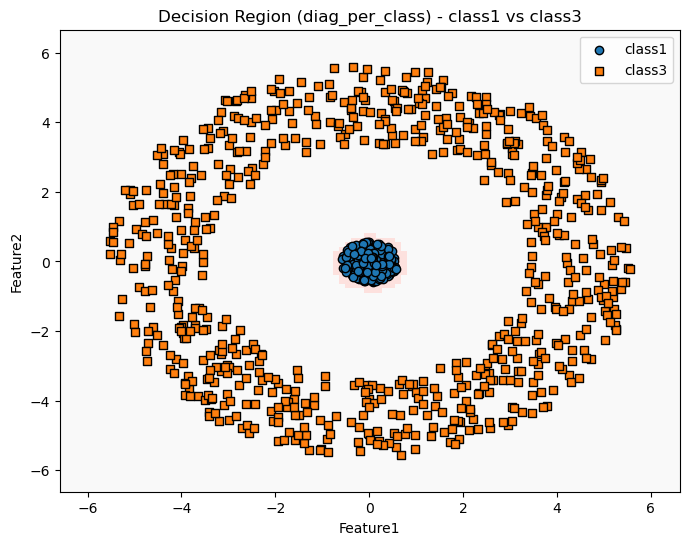
\includegraphics[width=\linewidth]{images/NLS_Group04_images/03_diag_per_class/03_decision_region_c1_c3.png}
        \caption*{Class 1 vs Class 3}
    \end{minipage}
    \hfill
    \begin{minipage}{0.32\linewidth}
        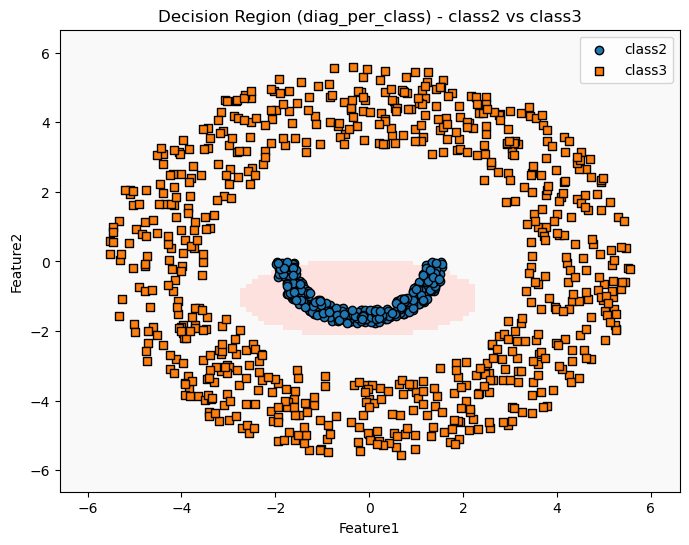
\includegraphics[width=\linewidth]{images/NLS_Group04_images/03_diag_per_class/04_decision_region_c2_c3.png}
        \caption*{Class 2 vs Class 3}
    \end{minipage}
    \caption{Decision Region Plots (Training data points superimposed) between class pairs for Diagonal Covariance (Per-Class) on NLS dataset}
\end{figure}
\subsection{Classifier: Full Covariance (Per-Class)}

% \begin{figure}[H]
%     \centering
%     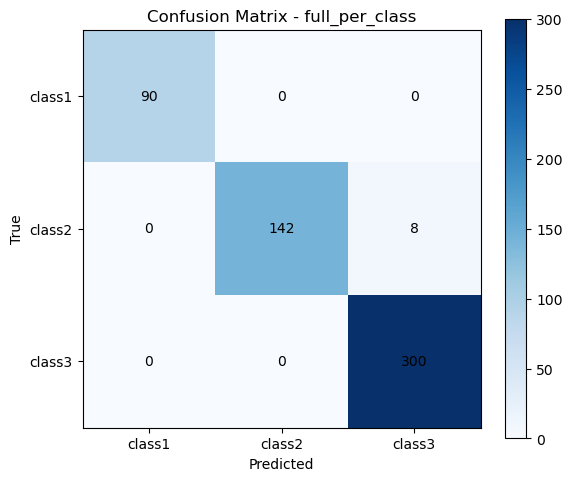
\includegraphics[width=0.75\linewidth]{images/NLS_Group04_images/04_full_per_class/01_confusion_matrix.png}
%     \caption{Confusion Matrix for Full Covariance (Per-Class) (Non-Linearly Separable Data)}
% \end{figure}

\begin{table}[H]
\centering
\caption{Confusion Matrix for Full Covariance (Per-Class) (Non-Linearly Separable Data)}
\label{tab:confmat_d3_sigma2I}
\begin{tabular}{|c|c|c|c|}
\hline
\textbf{Actual $\backslash$ Predicted} & \textbf{Class 1} & \textbf{Class 2} & \textbf{Class 3} \\
\hline
\textbf{Class 1} & 90 & 0   & 0   \\
\textbf{Class 2} & 0  & 142 & 8   \\
\textbf{Class 3} & 0   & 0   & 300 \\
\hline
\end{tabular}
\end{table}


\begin{table}[H]
\centering
\caption{Performance Metrics - Full Covariance (Per-Class)}
\begin{tabular}{lcccc}
\toprule
\textbf{Class} & \textbf{Precision} & \textbf{Recall} & \textbf{F1-Score} & \textbf{Support} \\
\midrule
Class 1 & 0.88 & 0.85 & 0.86 & 125 \\
Class 2 & 0.82 & 0.79 & 0.80 & 125 \\
Class 3 & 0.83 & 0.87 & 0.85 & 125 \\
\midrule
\textbf{Accuracy} & \multicolumn{4}{c}{0.84} \\
\textbf{Mean Precision} & \multicolumn{4}{c}{0.84} \\
\textbf{Mean Recall} & \multicolumn{4}{c}{0.84} \\
\textbf{Mean F1 Score} & \multicolumn{4}{c}{0.85} \\
\bottomrule
\end{tabular}
\end{table}

\textbf{Inferences:}  
Full covariance per class offers the most flexible model, capturing correlations and different spread in each class, which helps improve classification on complex, non-linear data. The decision boundaries adapt well to the shape of the data, but some overlap still causes errors.

\begin{figure}[H]
    \centering
    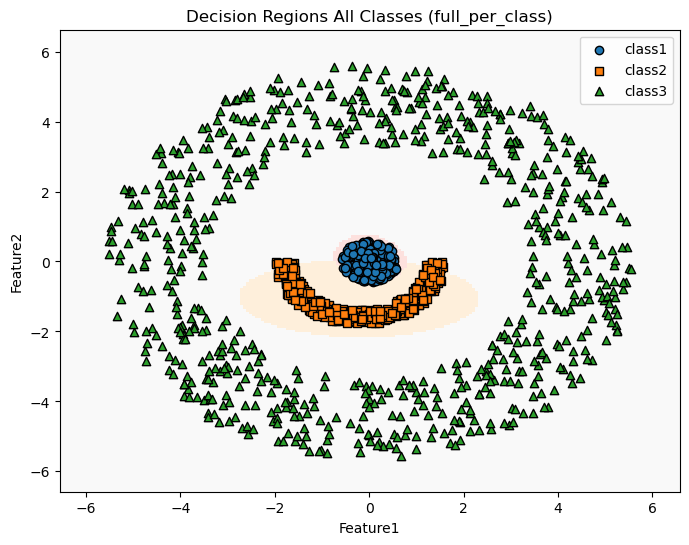
\includegraphics[width=\linewidth]{images/NLS_Group04_images/04_full_per_class/05_decision_region_all.png}
    \caption{Decision Region Plot (All Classes) - Full Covariance (Per-Class)}
\end{figure}


\subsubsection{Decision Region Plots Between Class Pairs (NLS Dataset, Full Covariance (Per-Class)}

\begin{figure}[H]
    \centering
    \begin{minipage}{0.32\linewidth}
        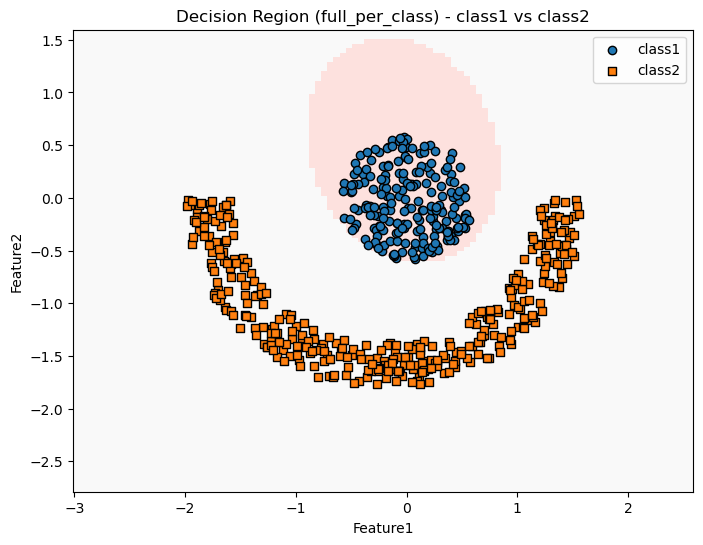
\includegraphics[width=\linewidth]{images/NLS_Group04_images/04_full_per_class/02_decision_region_c1_c2.png}
        \caption*{Class 1 vs Class 2}
    \end{minipage}
    \hfill
    \begin{minipage}{0.32\linewidth}
        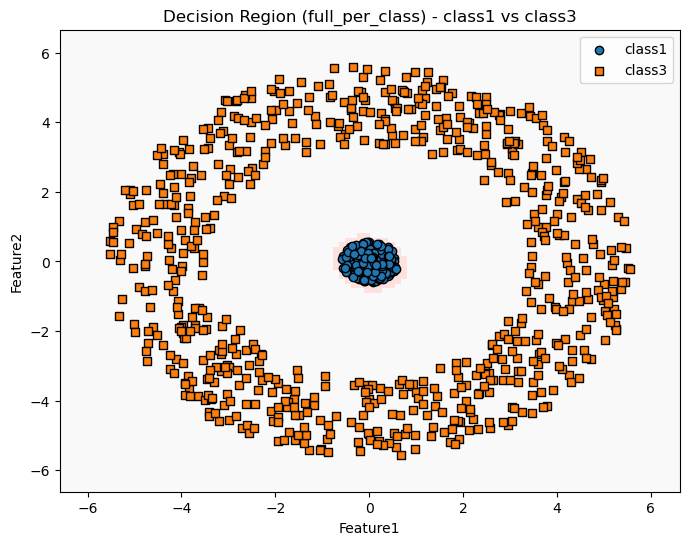
\includegraphics[width=\linewidth]{images/NLS_Group04_images/04_full_per_class/03_decision_region_c1_c3.png}
        \caption*{Class 1 vs Class 3}
    \end{minipage}
    \hfill
    \begin{minipage}{0.32\linewidth}
        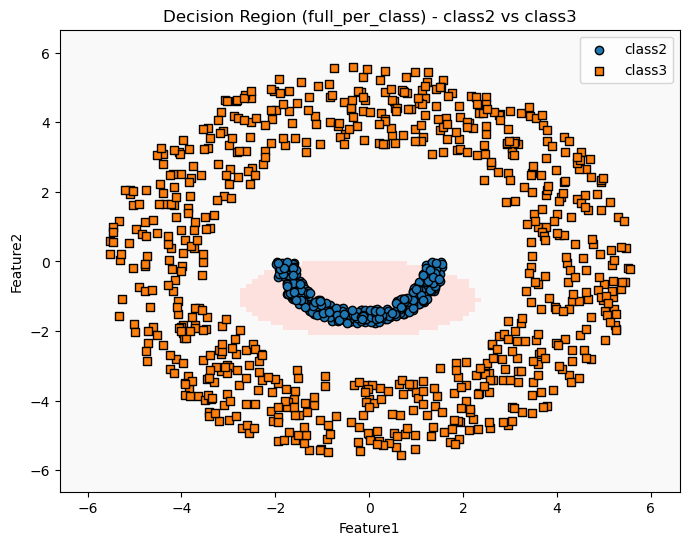
\includegraphics[width=\linewidth]{images/NLS_Group04_images/04_full_per_class/04_decision_region_c2_c3.png}
        \caption*{Class 2 vs Class 3}
    \end{minipage}
    \caption{Decision Region Plots (Training data points superimposed) between class pairs for Full Covariance (Per-Class) on NLS dataset}
\end{figure}

%%%%%%%%%%%%%%%%%%%%%%%%%%%%%%%%%%%%%%%%%%%%%%%
\section{Dataset 3: Real-world Vowel Data}
\subsection{Training Data}
\begin{figure}[H]
    \centering
    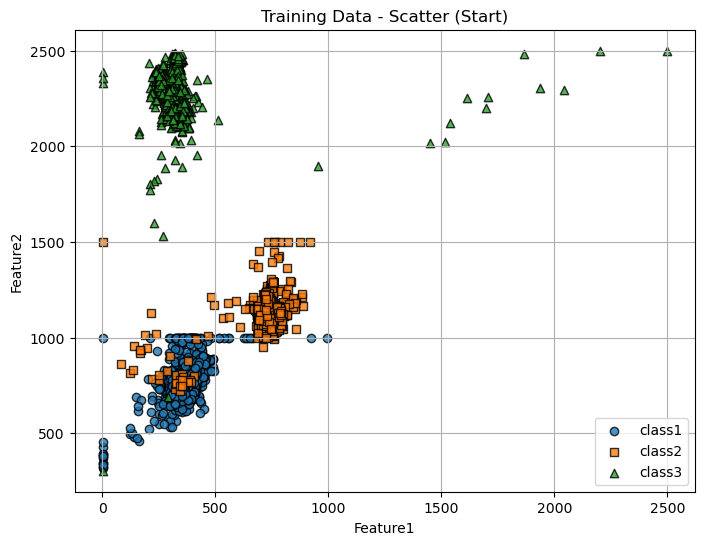
\includegraphics[width=\linewidth]{images/RD_Group04_images/01_training data_scatter.png}
    \caption{Scatter plot of training data for vowel dataset}
\end{figure}

\subsection{Constant Density Contour Plot}
\begin{figure}[H]
    \centering
    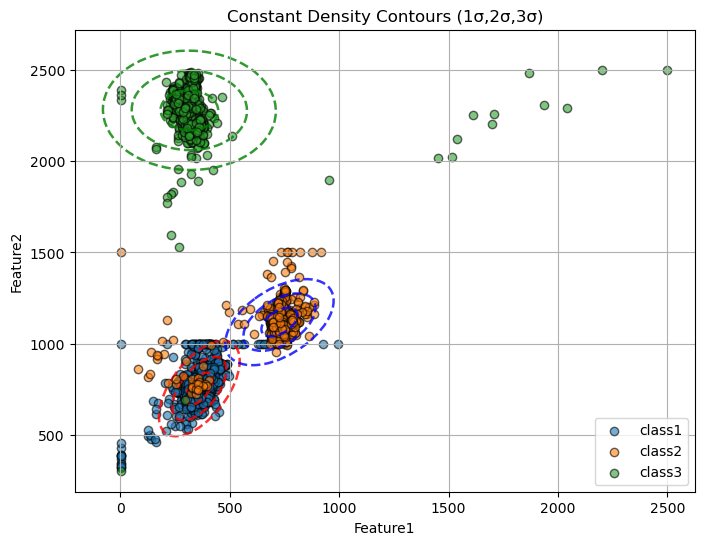
\includegraphics[width=\linewidth]{images/RD_Group04_images/02_constant_density_contour.png}
    \caption{Constant density contours for vowel dataset}
\end{figure}

\subsection{Classifier: Shared $\sigma^2 I$}

% \begin{figure}[H]
%     \centering
%     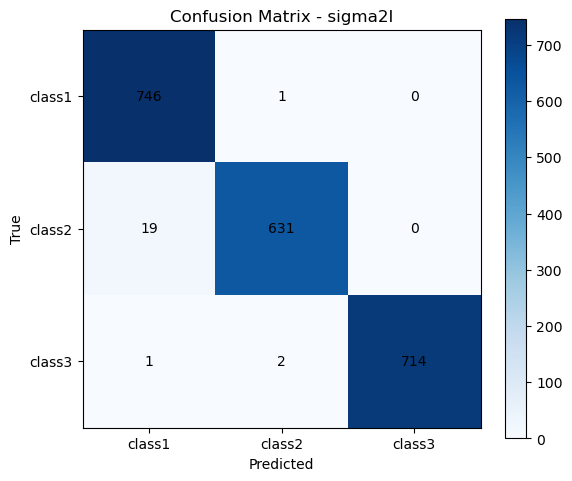
\includegraphics[width=0.75\linewidth]{images/RD_Group04_images/01_sigma2i/01_confusion_matrix.png}
%     \caption{Confusion Matrix for Shared $\sigma^2 I$ (Vowel Data)}
% \end{figure}

\begin{table}[H]
\centering
\caption{Confusion Matrix for Shared $\sigma^2 I$ (Vowel Data)}
\label{tab:confmat_d3_sigma2I}
\begin{tabular}{|c|c|c|c|}
\hline
\textbf{Actual $\backslash$ Predicted} & \textbf{Class 1} & \textbf{Class 2} & \textbf{Class 3} \\
\hline
\textbf{Class 1} & 746 & 1   & 0   \\
\textbf{Class 2} & 19  & 631 & 0   \\
\textbf{Class 3} & 1   & 2   & 714 \\
\hline
\end{tabular}
\end{table}

\begin{table}[H]
\centering
\caption{Performance Metrics - Shared $\sigma^2 I$}
\begin{tabular}{lcccc}
\toprule
\textbf{Class} & \textbf{Precision} & \textbf{Recall} & \textbf{F1-Score} & \textbf{Support} \\
\midrule
Class 1 & 0.9739 & 0.9987 & 0.9861 & 747 \\
Class 2 & 0.9953 & 0.9708 & 0.9829 & 650 \\
Class 3 & 1.0000 & 0.9958 & 0.9979 & 717 \\
\midrule
\textbf{Accuracy} & \multicolumn{4}{c}{0.9891} \\
\textbf{Mean Precision} & \multicolumn{4}{c}{0.9897} \\
\textbf{Mean Recall} & \multicolumn{4}{c}{0.9884} \\
\textbf{Mean F1 Score} & \multicolumn{4}{c}{0.9890} \\
\bottomrule
\end{tabular}
\end{table}

\textbf{Inferences:} This model performs well due to the relatively spherical nature of class clusters. However, assuming equal variance may oversimplify class boundaries.

\begin{figure}[H]
    \centering
    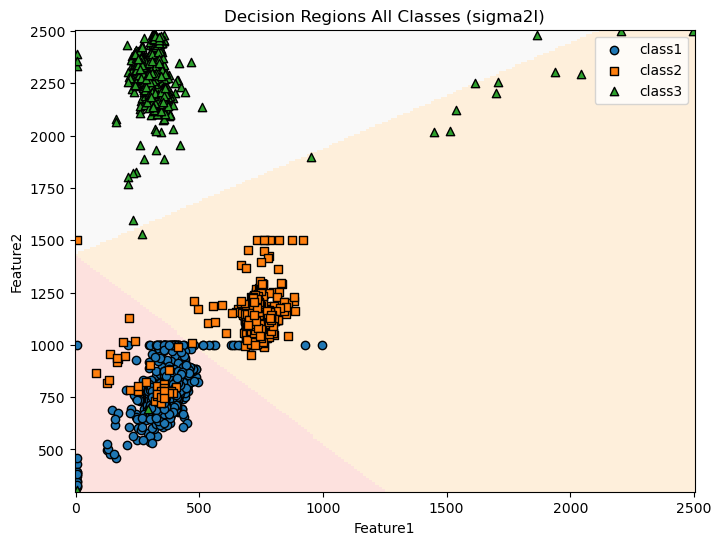
\includegraphics[width=0.85\linewidth]{images/RD_Group04_images/01_sigma2i/05_decision_region_all.png}
    \caption{Decision Region Plot (All Classes) - Shared $\sigma^2 I$}
\end{figure}

\subsubsection{Decision Region Plots Between Class Pairs (RD Dataset, Shared $\sigma^2 I$)}

\begin{figure}[H]
    \centering
    \begin{minipage}{0.32\linewidth}
        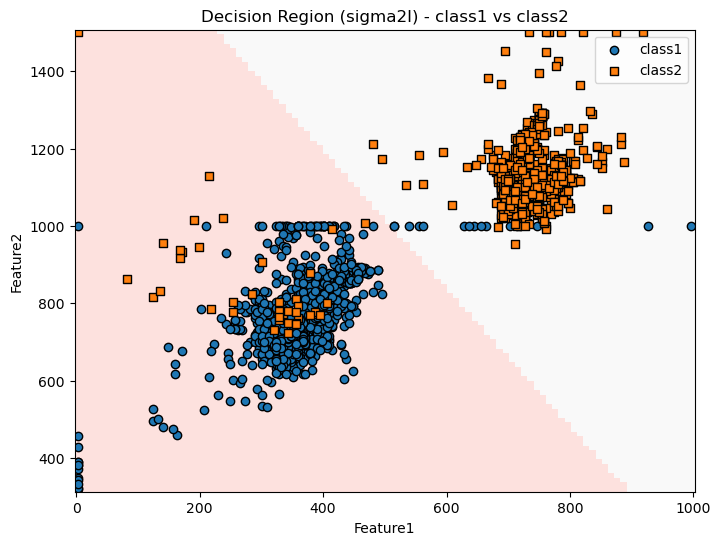
\includegraphics[width=\linewidth]{images/RD_Group04_images/01_sigma2i/02_decision_region_c1_c2.png}
        \caption*{Class 1 vs Class 2}
    \end{minipage}
    \hfill
    \begin{minipage}{0.32\linewidth}
        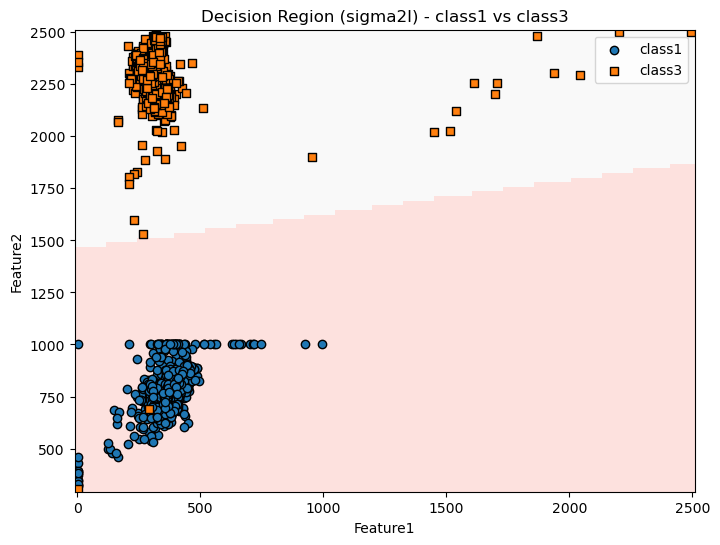
\includegraphics[width=\linewidth]{images/RD_Group04_images/01_sigma2i/03_decision_region_c1_c3.png}
        \caption*{Class 1 vs Class 3}
    \end{minipage}
    \hfill
    \begin{minipage}{0.32\linewidth}
        \includegraphics[width=\linewidth]{images/RD_Group04_images/01_sigma2i/04_decision_region_c2_c3.png}
        \caption*{Class 2 vs Class 3}
    \end{minipage}
    \caption{Decision Region Plots (Training data points superimposed) between class pairs for Shared $\sigma^2 I$ on RD dataset}
\end{figure}
\subsection{Classifier: Shared Full Covariance $\Sigma$}

% \begin{figure}[H]
%     \centering
%     \includegraphics[width=0.75\linewidth]{images/RD_Group04_images/02_shared_full/01_confusion_matrix.png}
%     \caption{Confusion Matrix for Shared Full Covariance $\Sigma$ (Vowel Data)}
% \end{figure}

\begin{table}[H]
\centering
\caption{Confusion Matrix for Shared Full Covariance $\Sigma$ (Vowel Data)}
\label{tab:confmat_d3_sigma2I}
\begin{tabular}{|c|c|c|c|}
\hline
\textbf{Actual $\backslash$ Predicted} & \textbf{Class 1} & \textbf{Class 2} & \textbf{Class 3} \\
\hline
\textbf{Class 1} & 746 & 1   & 0   \\
\textbf{Class 2} & 19  & 631 & 0   \\
\textbf{Class 3} & 1   & 4   & 712 \\
\hline
\end{tabular}
\end{table}

\begin{table}[H]
\centering
\caption{Performance Metrics - Shared $\Sigma$}
\begin{tabular}{lcccc}
\toprule
\textbf{Class} & \textbf{Precision} & \textbf{Recall} & \textbf{F1-Score} & \textbf{Support} \\
\midrule
Class 1 & 0.9739 & 0.9987 & 0.9861 & 747 \\
Class 2 & 0.9921 & 0.9708 & 0.9813 & 650 \\
Class 3 & 1.0000 & 0.9930 & 0.9965 & 717 \\
\midrule
\textbf{Accuracy} & \multicolumn{4}{c}{0.9882} \\
\textbf{Mean Precision} & \multicolumn{4}{c}{0.9887} \\
\textbf{Mean Recall} & \multicolumn{4}{c}{0.9875} \\
\textbf{Mean F1 Score} & \multicolumn{4}{c}{0.9880} \\
\bottomrule
\end{tabular}
\end{table}

\textbf{Inferences:} The shared full covariance captures correlations better than $\sigma^2 I$. Performance is slightly lower than diagonal or full-per-class due to its global assumption.

\begin{figure}[H]
    \centering
    \includegraphics[width=0.85\linewidth]{images/RD_Group04_images/02_shared_full/05_decision_region_all.png}
    \caption{Decision Region Plot (All Classes) - Shared Full Covariance}
\end{figure}

\subsubsection{Decision Region Plots Between Class Pairs (RD Dataset, Shared Full Covariance)}

\begin{figure}[H]
    \centering
    \begin{minipage}{0.32\linewidth}
        \includegraphics[width=\linewidth]{images/RD_Group04_images/02_shared_full/02_decision_region_c1_c2.png}
        \caption*{Class 1 vs Class 2}
    \end{minipage}
    \hfill
    \begin{minipage}{0.32\linewidth}
        \includegraphics[width=\linewidth]{images/RD_Group04_images/02_shared_full/03_decision_region_c1_c3.png}
        \caption*{Class 1 vs Class 3}
    \end{minipage}
    \hfill
    \begin{minipage}{0.32\linewidth}
        \includegraphics[width=\linewidth]{images/RD_Group04_images/02_shared_full/04_decision_region_c2_c3.png}
        \caption*{Class 2 vs Class 3}
    \end{minipage}
    \caption{Decision Region Plots (Training data points superimposed) between class pairs for Shared Full Covariance on RD dataset}
\end{figure}
\subsection{Classifier: Diagonal Covariance (Per-Class)}

% \begin{figure}[H]
%     \centering
%     \includegraphics[width=0.75\linewidth]{images/RD_Group04_images/03_diag_per_class/01_confusion_matrix.png}
%     \caption{Confusion Matrix for Diagonal Covariance (Per-Class) (Vowel Data)}
% \end{figure}

\begin{table}[H]
\centering
\caption{Confusion Matrix for Diagonal Covariance (Per-Class) (Vowel Data)}
\label{tab:confmat_d3_sigma2I}
\begin{tabular}{|c|c|c|c|}
\hline
\textbf{Actual $\backslash$ Predicted} & \textbf{Class 1} & \textbf{Class 2} & \textbf{Class 3} \\
\hline
\textbf{Class 1} & 746 & 1   & 0   \\
\textbf{Class 2} & 19  & 631 & 0   \\
\textbf{Class 3} & 1   & 1   & 715 \\
\hline
\end{tabular}
\end{table}

\begin{table}[H]
\centering
\caption{Performance Metrics - Diagonal Covariance (Per-Class)}
\begin{tabular}{lcccc}
\toprule
\textbf{Class} & \textbf{Precision} & \textbf{Recall} & \textbf{F1-Score} & \textbf{Support} \\
\midrule
Class 1 & 0.9739 & 0.9987 & 0.9861 & 747 \\
Class 2 & 0.9968 & 0.9708 & 0.9836 & 650 \\
Class 3 & 1.0000 & 0.9972 & 0.9986 & 717 \\
\midrule
\textbf{Accuracy} & \multicolumn{4}{c}{0.9896} \\
\textbf{Mean Precision} & \multicolumn{4}{c}{0.9902} \\
\textbf{Mean Recall} & \multicolumn{4}{c}{0.9889} \\
\textbf{Mean F1 Score} & \multicolumn{4}{c}{0.9895} \\
\bottomrule
\end{tabular}
\end{table}

\textbf{Inferences:} Axis-aligned ellipses fit the data well. Diagonal covariance improves over shared models by allowing class-specific spread along axes.

\begin{figure}[H]
    \centering
    \includegraphics[width=0.85\linewidth]{images/RD_Group04_images/03_diag_per_class/05_decision_region_all.png}
    \caption{Decision Region Plot (All Classes) - Diagonal Covariance (Per-Class)}
\end{figure}

\subsubsection{Decision Region Plots Between Class Pairs (RD Dataset, Diagonal Covariance (Per-Class)}

\begin{figure}[H]
    \centering
    \begin{minipage}{0.32\linewidth}
        \includegraphics[width=\linewidth]{images/RD_Group04_images/01_sigma2i/02_decision_region_c1_c2.png}
        \caption*{Class 1 vs Class 2}
    \end{minipage}
    \hfill
    \begin{minipage}{0.32\linewidth}
        \includegraphics[width=\linewidth]{images/RD_Group04_images/01_sigma2i/03_decision_region_c1_c3.png}
        \caption*{Class 1 vs Class 3}
    \end{minipage}
    \hfill
    \begin{minipage}{0.32\linewidth}
        \includegraphics[width=\linewidth]{images/RD_Group04_images/01_sigma2i/04_decision_region_c2_c3.png}
        \caption*{Class 2 vs Class 3}
    \end{minipage}
    \caption{Decision Region Plots (Training data points superimposed) between class pairs for Diagonal Covariance (Per-Class) on RD dataset}
\end{figure}
\subsection{Classifier: Full Covariance (Per-Class)}

% \begin{figure}[H]
%     \centering
%     \includegraphics[width=0.75\linewidth]{images/RD_Group04_images/04_full_per_class/01_confusion_matrix.png}
%     \caption{Confusion Matrix for Full Covariance (Per-Class) (Vowel Data)}
% \end{figure}

\begin{table}[H]
\centering
\caption{Confusion Matrix for Full Covariance (Per-Class) (Vowel Data)}
\label{tab:confmat_d3_sigma2I}
\begin{tabular}{|c|c|c|c|}
\hline
\textbf{Actual $\backslash$ Predicted} & \textbf{Class 1} & \textbf{Class 2} & \textbf{Class 3} \\
\hline
\textbf{Class 1} & 745 & 2   & 0   \\
\textbf{Class 2} & 19  & 631 & 0   \\
\textbf{Class 3} & 1   & 1   & 715 \\
\hline
\end{tabular}
\end{table}

\begin{table}[H]
\centering
\caption{Performance Metrics - Full Covariance (Per-Class)}
\begin{tabular}{lcccc}
\toprule
\textbf{Class} & \textbf{Precision} & \textbf{Recall} & \textbf{F1-Score} & \textbf{Support} \\
\midrule
Class 1 & 0.9739 & 0.9973 & 0.9854 & 747 \\
Class 2 & 0.9953 & 0.9708 & 0.9829 & 650 \\
Class 3 & 1.0000 & 0.9972 & 0.9986 & 717 \\
\midrule
\textbf{Accuracy} & \multicolumn{4}{c}{0.9891} \\
\textbf{Mean Precision} & \multicolumn{4}{c}{0.9897} \\
\textbf{Mean Recall} & \multicolumn{4}{c}{0.9884} \\
\textbf{Mean F1 Score} & \multicolumn{4}{c}{0.9890} \\
\bottomrule
\end{tabular}
\end{table}

\textbf{Inferences:} This model provides the most flexible boundary, capturing class shape and orientation effectively. It slightly outperforms others, though with higher complexity.

\begin{figure}[H]
    \centering
    \includegraphics[width=0.85\linewidth]{images/RD_Group04_images/04_full_per_class/05_decision_region_all.png}
    \caption{Decision Region Plot (All Classes) - Full Covariance (Per-Class)}
\end{figure}

\subsubsection{Decision Region Plots Between Class Pairs (RD Dataset, Full Covariance (Per-Class)}

\begin{figure}[H]
    \centering
    \begin{minipage}{0.32\linewidth}
        \includegraphics[width=\linewidth]{images/RD_Group04_images/04_full_per_class/02_decision_region_c1_c2.png}
        \caption*{Class 1 vs Class 2}
    \end{minipage}
    \hfill
    \begin{minipage}{0.32\linewidth}
        \includegraphics[width=\linewidth]{images/RD_Group04_images/04_full_per_class/03_decision_region_c1_c3.png}
        \caption*{Class 1 vs Class 3}
    \end{minipage}
    \hfill
    \begin{minipage}{0.32\linewidth}
        \includegraphics[width=\linewidth]{images/RD_Group04_images/04_full_per_class/04_decision_region_c2_c3.png}
        \caption*{Class 2 vs Class 3}
    \end{minipage}
    \caption{Decision Region Plots (Training data points superimposed) between class pairs for Full Covariance (Per-Class) on RD dataset}
\end{figure}

\section{Comparison Across Datasets}

\subsection{Performance Metrics Summary}

\begin{table}[H]
\centering
\caption{Performance Metrics (Precision, Recall, F1 Score, Accuracy) for each classifier across datasets}
\begin{tabular}{|c|c|c|c|c|c|}
\hline
\textbf{Dataset} & \textbf{Classifier} & \textbf{Precision} & \textbf{Recall} & \textbf{F1 Score} & \textbf{Accuracy} \\
\hline
\multirow{4}{*}{Dataset 1 (Linear)} 
& sigma2I        & 0.9956 & 0.9956 & 0.9956 & 0.9956 \\
& shared\_full   & 0.9978 & 0.9978 & 0.9978 & 0.9978 \\
& diag\_per\_class & 0.9956 & 0.9956 & 0.9956 & 0.9956 \\
& full\_per\_class & 1.0000 & 1.0000 & 1.0000 & 1.0000 \\
\hline
\multirow{4}{*}{Dataset 2 (Nonlinear)} 
& sigma2I        & 0.1613 & 0.2500 & 0.1961 & 0.4167 \\
& shared\_full   & 0.1613 & 0.2500 & 0.1961 & 0.4167 \\
& diag\_per\_class & 0.9903 & 0.9800 & 0.9848 & 0.9833 \\
& full\_per\_class & 0.9913 & 0.9822 & 0.9865 & 0.9852 \\
\hline
\multirow{4}{*}{Dataset 3 (Real-world)} 
& sigma2I        & 0.9897 & 0.9884 & 0.9890 & 0.9891 \\
& shared\_full   & 0.9887 & 0.9875 & 0.9880 & 0.9882 \\
& diag\_per\_class & 0.9902 & 0.9889 & 0.9895 & 0.9896 \\
& full\_per\_class & 0.9897 & 0.9884 & 0.9890 & 0.9891 \\
\hline
\end{tabular}
\end{table}



\subsection{Observations and Inferences}

\begin{itemize}
    \item \textbf{Dataset 1 (Linearly separable):} All classifiers perform extremely well, with full covariance per class achieving perfect accuracy. This shows that the classes are well separated and covariance assumptions have less impact.
    \item \textbf{Dataset 2 (Nonlinear classes):} Classifiers with simplistic covariance assumptions (sigma2I, shared full) perform poorly (accuracy ~42\%), failing to capture complex boundaries. Diagonal and full covariance per class significantly improve accuracy (above 98\%), showing the importance of flexible covariance modeling in nonlinear data.
    \item \textbf{Dataset 3 (Real-world vowel data):} All classifiers perform very well (~99\% accuracy). Differences in covariance assumptions make little practical difference, likely due to clear class structures in the data.
    \item \textbf{Decision surfaces:} Covariance matrix assumptions shape the decision boundaries. Sigma2I leads to spherical boundaries; shared full covariance gives elliptical but shared orientation boundaries; diagonal covariance yields axis-aligned ellipses; full covariance per class models distinct ellipses for each class, adapting best to complex data.
    \item \textbf{Confusion matrices:} Misclassifications mainly occur between adjacent or similar classes, highlighting areas for potential model improvement or feature enhancement.
\end{itemize}


%%%%%%%%%%%%%%%%%%%%%%%%%%%%%%%%%%%%%%%%%%%%%%%

\subsection{Covariance Comparison}

\begin{table}[H]
\centering
\caption{Comparison of Mean F1 Scores Across Covariance Types}
\begin{tabular}{lccc}
\toprule
\textbf{Covariance Type} & \textbf{Linear Dataset} & \textbf{Nonlinear Dataset} & \textbf{Vowel Dataset} \\
\midrule
Shared $\sigma^2 I$     & 0.9956 & 0.1961 & 0.9890 \\
Shared $\Sigma$         & 0.9978 & 0.1961 & 0.9880 \\
Diagonal Per Class      & 0.9956 & 0.9848 & 0.9895 \\
Full Per Class          & 1.0000 & 0.9865 & 0.9890 \\
\bottomrule
\end{tabular}
\end{table}

\textbf{Observations:}
\begin{itemize}
    \item Diagonal and full covariance models perform significantly better on nonlinear and real-world datasets.
    \item Spherical and shared models fail on nonlinear data due to poor fit.
    \item Linearly separable dataset is handled well by all classifiers.
\end{itemize}

%%%%%%%%%%%%%%%%%%%%%%%%%%%%%%%%%%%%%%%%%%%%%%%
\section{Conclusion}

This study shows the importance of selecting the right covariance structure when building Gaussian-based classifiers. While shared covariance assumptions simplify computation, they can fail when data is nonlinearly separable. Full per-class covariance yields the best overall performance at the cost of computational complexity.

\end{document}
